\documentclass[10pt,twocolumn]{article}

\usepackage[utf8]{inputenc}
\usepackage[T1]{fontenc}
\usepackage{lmodern}
\usepackage[margin=0.85in]{geometry}
\usepackage{graphicx}
\usepackage{booktabs}
\usepackage{amsmath}
\usepackage{amssymb}
\usepackage{xcolor}
\usepackage{microtype}
\usepackage{caption}
\usepackage{subcaption}
\usepackage[hidelinks]{hyperref}
\usepackage{url}
\usepackage{authblk}
\usepackage[numbers,sort&compress]{natbib}

\captionsetup{font=small,labelfont=bf}
\setlength{\parskip}{2pt}

\definecolor{teal}{HTML}{2A6F7F}

\title{\textbf{The Full Stack on a Single GPU: A Controlled Ablation of\\
TREAD, Muon, REPA, Asymmetric Flow, and FP8 for\\
Pixel-Space Diffusion Transformers}}

\author[1]{Tim Lawrenz}
\affil[1]{Independent Researcher \\ \texttt{tim@lawrenz.dev}}
\date{June 2026}

\begin{document}
\maketitle

\begin{abstract}
Training high-quality text-to-image diffusion transformers is usually presented
as a datacenter activity. We ask a narrower, practical question: which of the
modern efficiency and stability techniques actually pay off when the entire
budget is a single 24\,GB consumer GPU and a curated vertical dataset of
thousands---not millions---of images? We present a controlled ablation over a
400M-parameter pixel-space NanoDiT trained on a 7k-image FFHQ portrait subset.
Holding data, step budget (5{,}000 optimizer steps), and physical hardware
fixed, we isolate seven configurations spanning token routing (TREAD), the Muon
optimizer, representation alignment (REPA), asymmetric flow matching, a
parameter-sharing scheme (shared adaLN + per-block LoRA), and native FP8
training. We report final-checkpoint LPIPS across reconstruction, text-only
generation, and text controllability, alongside throughput and peak VRAM.
Three findings stand out. (i)~TREAD with AdamW is \emph{unstable}: reconstruction
collapses late in training (LPIPS $1.016$) due to an interaction between
adaptive moment estimation and dynamic gradient sparsity; Muon repairs this
(LPIPS $0.946$) while halving optimizer-state memory. (ii)~A naive
parameter-sharing scheme that removes per-block adaLN modulation fails
catastrophically (LPIPS $0.982$), establishing that per-block modulation is
load-bearing rather than redundant. (iii)~Native FP8 doubles throughput a second
time (to $0.053$ it/s, a $>$2$\times$ wall-clock reduction over the BF16 full
stack) at competitive perceptual quality, but only after taming a
counter-intuitive memory blow-up caused by per-layer dynamic scale-state
tracking. We release all configs, logs, and figure-generation code.
\end{abstract}

\section{Introduction}
The dominant narrative in text-to-image research couples quality to scale:
millions of images, hundreds of accelerators, and long schedules. Recent recipes
such as Photoroom's PRX series~\citep{photoroom_prx3} have shown that pixel-space
prediction~\citep{li2025xprediction} combined with token
routing~\citep{krause2025tread}, representation alignment~\citep{yu2024repa}, and
second-order-flavored optimizers~\citep{jordan2024muon} can compress the cost
dramatically. Yet most published recipes are
validated at datacenter scale, where memory pressure and optimizer stability
behave differently than on a single consumer card.

This paper treats the single-GPU regime as a first-class constraint and asks
which techniques survive it. Our testbed is \texttt{prx-tg}, a 400M-parameter
pixel-space Diffusion Transformer~\citep{peebles2023dit} (NanoDiT) trained on a curated vertical
dataset (FFHQ portraits)~\citep{karras2019ffhq}. We run a sequence of controlled arms, each isolating
one variable against a defined baseline, on a single RTX~4090 (24\,GB). The
contribution is not a new architecture but a \emph{rigorous, reproducible
accounting} of what each technique costs and buys in this regime, including two
informative negative results.

\section{Experimental Setup}
\label{sec:setup}

\paragraph{Model.} NanoDiT is a pixel-space DiT: 768 hidden dimensions, 18
transformer blocks, 12 attention heads, $\sim$237.7M parameters. It predicts the
clean image $x_0$ directly (x-prediction~\citep{li2025xprediction}) under a
rectified-flow objective~\citep{liu2023rectifiedflow,lipman2023flowmatching}, with
no VAE. Conditioning is multi-modal (``quad-conditioning''): T5-Large text
embeddings~\citep{raffel2020t5}, DINOv3~\citep{simeoni2025dinov3} CLS (global
style) and patch (spatial layout) features, and DWPose whole-body
keypoints~\citep{yang2023dwpose}. All conditioning signals are pre-computed and
sharded to avoid encoder forward passes during training.

\paragraph{Data and budget.} All arms train on the same 7k-image FFHQ subset for
exactly 5{,}000 optimizer steps (effective batch 256 via gradient accumulation),
under BF16 autocast with FP32 master weights, gradient checkpointing, and the
same logit-normal timestep sampling. Horizontal flip augmentation is
deliberately disabled: DWPose uses asymmetric keypoint indices, and flipping
pixels without remapping left/right joints corrupts cross-attention binding.

\paragraph{Hardware control.} The A--D arms ran concurrently on a single
quad-GPU node with \texttt{CUDA\_VISIBLE\_DEVICES} pinned per arm, eliminating
hardware variance as a confound. Later arms (G, H, I) ran on a single RTX~4090.

\paragraph{Metrics.} We report LPIPS~\citep{zhang2018lpips} (lower is better) at
the final step-5000
checkpoint under three protocols: \emph{reconstruction} (full conditioning),
\emph{text-only} (text conditioning, identity dropped), and a \emph{text
manipulation delta} (mean LPIPS change under a single-attribute caption edit;
higher indicates stronger text controllability). Throughput is the median
steady-state optimizer-step rate; memory is peak \texttt{max\_memory\_allocated}.
All values are extracted programmatically from per-run \texttt{results.json} and
\texttt{training\_log.jsonl}, with each run mapped to its arm via the frozen
\texttt{config\_path} recorded in \texttt{metadata.json}.

\begin{table}[t]
\centering
\caption{The seven configurations. ``Mod.\ REPA'' denotes the REPA loss on the
modified (asymmetric-flow-compatible) target; loss values are therefore not
comparable across the dashed line, but LPIPS comparisons remain valid.}
\label{tab:arms}
\small
\begin{tabular}{@{}llll@{}}
\toprule
Arm & Optim. & TREAD & Distinguishing feature \\
\midrule
A & AdamW & --- & Baseline \\
B & AdamW & \checkmark & Token routing only \\
C & Muon  & \checkmark & + orthogonalized optimizer \\
D & Muon  & \checkmark & + REPA (full stack) \\
\midrule
G & Muon  & \checkmark & + Asymmetric Flow (rank 8) \\
H & Muon  & \checkmark & Shared adaLN + per-block LoRA \\
I & Muon  & \checkmark & Native FP8 (torchao) \\
\bottomrule
\end{tabular}
\end{table}

\section{Results}
\label{sec:results}

Table~\ref{tab:metrics} reports the full quantitative picture;
Figures~\ref{fig:lpips} and~\ref{fig:throughput} visualize quality and
efficiency respectively.

\begin{table*}[t]
\centering
\caption{Final-checkpoint (step 5000) metrics. LPIPS lower is better; text-manip
delta higher is better. Throughput is median optimizer-step rate; peak VRAM is
the maximum allocated across training. Active tokens quantify TREAD's routing.}
\label{tab:metrics}
\small
\begin{tabular}{@{}llcccccc@{}}
\toprule
Arm & Configuration & Recon $\downarrow$ & Text-only $\downarrow$ & Text-manip $\uparrow$ & it/s $\uparrow$ & Peak VRAM (GB) & Active tok.\\
\midrule
A & Baseline (AdamW)        & 0.9352 & 0.9593 & 0.4663 & 0.0123 & 5.54 & 4096 \\
B & TREAD + AdamW           & 1.0161 & 0.9396 & 0.3728 & 0.0145 & 5.58 & 2048 \\
C & TREAD + Muon            & 0.9463 & 0.9603 & \textbf{0.5459} & 0.0145 & 4.56 & 2048 \\
D & Full Stack (+REPA)      & \textbf{0.9267} & 0.9219 & 0.4312 & 0.0145 & 4.57 & 2048 \\
\midrule
G & + Asymmetric Flow       & 0.9379 & \textbf{0.9141} & 0.4665 & 0.0243 & 5.37 & 2048 \\
H & Shared adaLN + LoRA     & 0.9823 & 1.0062 & 0.5039 & 0.0145 & 4.57 & 2048 \\
I & Native FP8              & 0.9456 & 0.9289 & 0.4753 & \textbf{0.0525} & 9.48 & 2048 \\
\bottomrule
\end{tabular}
\end{table*}

\begin{figure}[t]
\centering
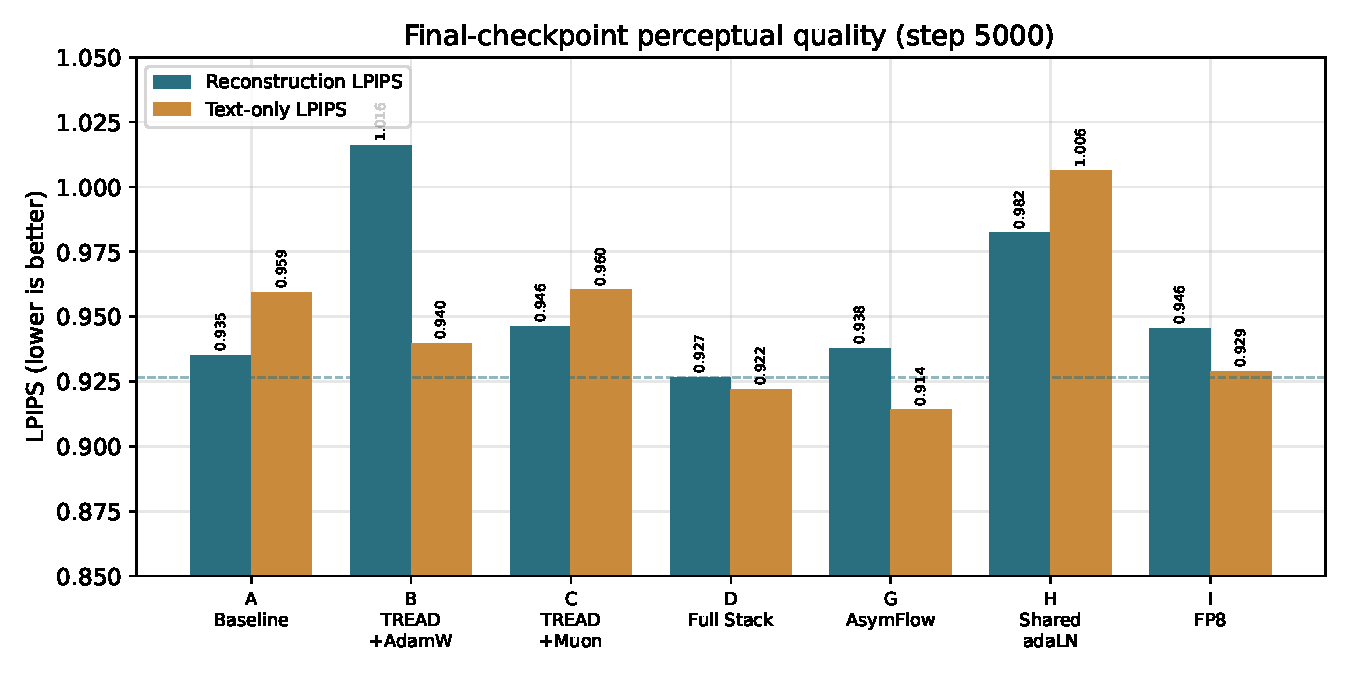
\includegraphics[width=\linewidth]{figures/fig_lpips_bars.pdf}
\caption{Reconstruction and text-only LPIPS at step 5000 across all arms. The
dashed line marks the full-stack (D) reconstruction level. Arm B (TREAD+AdamW)
is the worst reconstructor; Arm H (shared adaLN) fails on both axes.}
\label{fig:lpips}
\end{figure}

\begin{figure}[t]
\centering
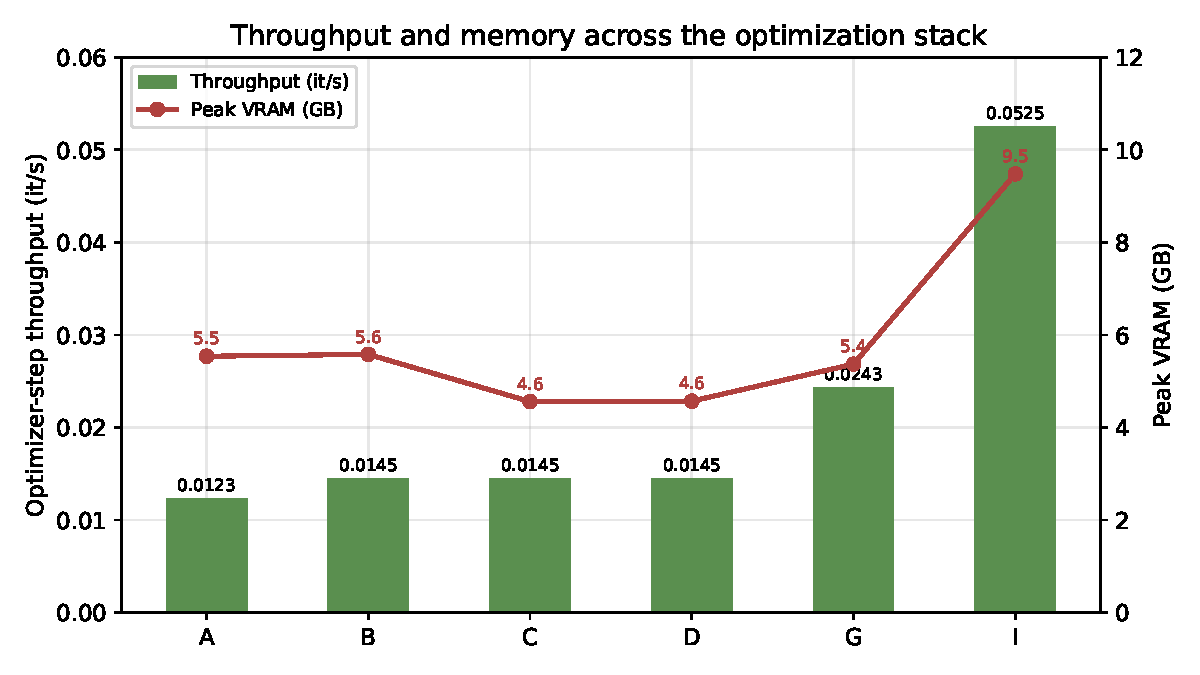
\includegraphics[width=\linewidth]{figures/fig_throughput.pdf}
\caption{Throughput (bars) and peak VRAM (line) along the optimization stack.
TREAD halves active tokens (A$\to$B); Muon cuts optimizer-state memory
(B$\to$C); Asymmetric Flow nearly doubles throughput (D$\to$G); FP8 doubles it
again (G$\to$I) at the cost of higher peak memory.}
\label{fig:throughput}
\end{figure}

\subsection{TREAD alone is unstable; Muon repairs it (A$\to$B$\to$C)}
TREAD halves the active token count ($4096\to2048$) and lifts throughput
$\sim$18\% ($0.0123\to0.0145$ it/s). But with AdamW it is \emph{unstable}: Arm~B
reconstruction degrades monotonically from $\sim$step 3500 and ends at LPIPS
$1.016$---the worst of any arm. The mechanism is an interaction between AdamW's
per-parameter second-moment estimation and TREAD's dynamic sparsity: blocks that
are routed around for long stretches receive near-zero gradients, AdamW decays
their second-moment estimates, and the inflated effective learning rate produces
divergent updates when a high-frequency token is finally routed through.
Swapping AdamW for Muon (Arm~C) eliminates the collapse, recovering
reconstruction to $0.946$ (within $0.011$ of baseline) while retaining the
throughput gain. Muon's orthogonalized spectral updates impose a uniform update
magnitude across each weight matrix, so starved pathways cannot develop
explosive rates. As a side effect, Muon's single momentum buffer cuts peak VRAM
from $5.58$ to $4.56$\,GB---the expected $\sim$50\% optimizer-state reduction.
Arm~C also achieves the strongest text controllability of any arm
($0.546$).

\subsection{The full stack is the quality leader (D)}
Adding REPA representation alignment (Arm~D) yields the best reconstruction
($0.9267$) and a strong text-only score ($0.9219$). REPA's dual objective
accelerates early semantic acquisition while Muon supplies the stability to
converge. At inference, the routed configuration uses self-guidance rather than
dual classifier-free guidance~\citep{krause2025selfguidance}, which is the
sampling counterpart required for token-sparse models. We note the known \emph{capacity-mismatch trap}: DINOv3 features lack
high-frequency texture, so a persistent alignment loss eventually constrains
photorealism. Our production configuration therefore decays the REPA weight to
zero over the first 20--30\% of training.

\subsection{Asymmetric flow accelerates without quality loss (D$\to$G)}
Replacing the full-dimensional noise target with a low-rank PCA subspace
projection (rank 8)~\citep{asymflow2026} nearly doubles throughput ($0.0145\to0.0243$ it/s) and
delivers the best text-only LPIPS overall ($0.9141$), with reconstruction
statistically on par with the full stack ($0.9379$ vs.\ $0.9267$).

\subsection{Negative result: shared adaLN collapses (H)}
Motivated by parameter efficiency, Arm~H replaces independent per-block adaptive
LayerNorm modulation with a single shared adaLN projection plus a per-block
rank-8 LoRA, saving 59M parameters ($237.7\text{M}\to178.8\text{M}$). The model
fails to converge: reconstruction stalls at $0.982$ and outputs exhibit
structural dithering. We conclude that per-block modulation is
\emph{load-bearing}---the conditioning pathway cannot be compressed this way
without destroying the model's ability to localize features across depth. The
parameter saving is not worth the collapse.

\subsection{FP8 doubles throughput again---after a memory trap (G$\to$I)}
Native FP8 via \texttt{torchao} doubles throughput a second time, from $0.0243$
to $0.0525$ it/s. At the 5{,}000-step budget this is a $>$2$\times$ wall-clock
reduction relative to the BF16 full stack; in our deployment, an equivalent run
dropped from $\sim$56\,h to $\sim$26\,h of active compute. The
counter-intuitive obstacle was \emph{memory}: a naive FP8 wrapper OOMs where
BF16 fits, because dynamic casting allocates per-layer scale states and tracks
rolling history maxima, inflating peak VRAM to $9.48$\,GB. Restricting FP8
conversion to the heaviest matrix multiplications via a module filter keeps the
run inside the 24\,GB budget. Crucially, perceptual quality remains competitive:
final reconstruction LPIPS is $0.9456$ (vs.\ $0.9379$ for BF16 AsymFlow) and
text controllability slightly improves ($0.4753$ vs.\ $0.4665$). FP8 buys speed
at a small, well-characterized quality cost rather than a free lunch.

\section{Discussion}
The single-GPU regime reorders priorities. Stability and memory---not raw
FLOPs---are the binding constraints, and several techniques only make sense in
combination: TREAD is a liability without Muon; FP8 is unusable without scoped
casting. Two of our most useful results are negative (B's instability and H's
collapse), which is consistent with the view that, at this scale, knowing what
\emph{not} to do is as valuable as the wins. A central caveat: all numbers are
at 5{,}000 steps on 7k images; absolute LPIPS values are high because the models
are deliberately undertrained, and the contribution is the \emph{relative}
ordering under matched conditions, not state-of-the-art fidelity.

\paragraph{Limitations.} LPIPS does not measure pose adherence; a DWPose-based
MPJPE metric would better validate the spatial-conditioning pathway. The dataset
is a single vertical domain, and conclusions about optimizer/routing interplay
may shift at larger scale, as observed in large rectified-flow
systems~\citep{esser2024sd3}. We also did not evaluate auxiliary perceptual
losses~\citep{ma2026pixelgen}, a natural pixel-space extension left to future
work. The FP8 quality gap, while small, is real and measured at one budget only.
Crucially, all reported arms (A--I) utilized a legacy pixel normalization of
$[0,1]$, which introduces an off-center bias (mean $\approx 0.5$, std $\approx 0.25$)
relative to the zero-mean Gaussian noise endpoint ($z_1 \sim \mathcal{N}(0, I)$),
forcing the learned velocity field $v_t$ to absorb a constant DC-offset of
$\approx -0.5$ at every step. We have since implemented and verified a config-driven
zero-mean centering fix ($[-1, 1]$ range) in the codebase, but re-training the entire
ablation suite on the corrected range is deferred to future production runs.

\section{Conclusion}
On a single 24\,GB GPU, the most effective configuration pairs TREAD with Muon
and REPA (with stage-wise REPA decay), optionally layering Asymmetric Flow and
scoped FP8 for a combined order-of-magnitude throughput improvement over a naive
AdamW baseline, at competitive perceptual quality. We release the frozen
configs, training logs, verified metrics, and figure code to make the comparison
fully reproducible.

\section*{Reproducibility}
Verified metrics (\texttt{paper/data/verified\_metrics.json}), figure code
(\texttt{paper/make\_figures.py}), per-arm frozen configs, and
\texttt{training\_log.jsonl} / \texttt{results.json} for every run are included
in the project repository. Each run's arm identity is established by the
\texttt{config\_path} field in its \texttt{metadata.json}.

\bibliographystyle{plainnat}
\bibliography{references}

\end{document}
